%------------------------------------------------------------------------------
% Template file for the submission of papers to IUCr journals in LaTeX2e
% using the iucr document class
% Copyright 1999-2013 International Union of Crystallography
% Version 1.6 (28 March 2013)
%------------------------------------------------------------------------------

\documentclass[preprint]{iucr}              % DO NOT DELETE THIS LINE

     %-------------------------------------------------------------------------
     % Information about journal to which submitted
     %-------------------------------------------------------------------------
     \journalcode{M}              % Indicate the journal to which submitted
                                  %   A - Acta Crystallographica Section A
                                  %   B - Acta Crystallographica Section B
                                  %   C - Acta Crystallographica Section C
                                  %   D - Acta Crystallographica Section D
                                  %   E - Acta Crystallographica Section E
                                  %   F - Acta Crystallographica Section F
                                  %   J - Journal of Applied Crystallography
                                  %   M - IUCrJ
                                  %   S - Journal of Synchrotron Radiation

\usepackage{amsmath}
\usepackage[version=4]{mhchem}
\usepackage{siunitx}
\usepackage{nicematrix}
\usepackage{url}
\begin{document}                  % DO NOT DELETE THIS LINE

     %-------------------------------------------------------------------------
     % The introductory (header) part of the paper
     %-------------------------------------------------------------------------

     % The title of the paper. Use \shorttitle to indicate an abbreviated title
     % for use in running heads (you will need to uncomment it).

\title{A transferable quantum mechanical energy model for intermolecular interactions using a single empirical parameter}
%\shorttitle{Short Title}

     % Authors' names and addresses. Use \cauthor for the main (contact) author.
     % Use \author for all other authors. Use \aff for authors' affiliations.
     % Use lower-case letters in square brackets to link authors to their
     % affiliations; if there is only one affiliation address, remove the [a].

\cauthor[a]{Peter R.}{Spackman}{peter.spackman@curtin.edu.au}{}
\author[b]{Mark A.}{Spackman}
\author[a]{Julian D.}{Gale}

\aff[a]{School of Molecular and Life Sciences, Curtin University, Perth, Western Australia 6845, \country{Australia}}
\aff[b]{School of Molecular Sciences, University of Western Australia, Perth, Western Australia 6009, \country{Australia}}

     % Use \shortauthor to indicate an abbreviated author list for use in
     % running heads (you will need to uncomment it).

%\shortauthor{Soape, Author and Doe}

     % Use \vita if required to give biographical details (for authors of
     % invited review papers only). Uncomment it.

%\vita{Author's biography}

     % Keywords (required for Journal of Synchrotron Radiation only)
     % Use the \keyword macro for each word or phrase, e.g. 
     % \keyword{X-ray diffraction}\keyword{muscle}

%\keyword{keyword}

     % PDB and NDB reference codes for structures referenced in the article and
     % deposited with the Protein Data Bank and Nucleic Acids Database (Acta
     % Crystallographica Section D). Repeat for each separate structure e.g
     % \PDBref[dethiobiotin synthetase]{1byi} \NDBref[d(G$_4$CGC$_4$)]{ad0002}

%\PDBref[optional name]{refcode}
%\NDBref[optional name]{refcode}

\maketitle                        % DO NOT DELETE THIS LINE

\begin{synopsis}
Supply a synopsis of the paper for inclusion in the Table of Contents.
\end{synopsis}

\begin{abstract}
The calculation of intermolecular interactions in molecular crystals using model energies
provides a unified route to understanding the complex interplay of driving forces in 
crystallisation, elastic properties and more.
We present a new single parameter interaction energy model (CE-1p) extending the previous CrystalExplorer energy model,
calibrated using DFT calculations at the $\omega$B97M-V/def2-QZVP level over 1157 intermolecular interactions from 147 crystal structures.
The new model incorporates an improved treatment of dispersion interactions and polarisabilities
using the eXchange-hole Dipole Model (XDM), along with the use of Effective Core Potentials (ECPs) 
facilitating application to molecules containing elements across the periodic table (from \ce{H} to \ce{Rn}).
This new model is validated against high-level reference data, with outstanding performance,
comparable to state-of-the-art DFT methods for molecular crystal lattice energies over the X23 set ($\text{MAD} = 3.6$ kJ/mol)
and for intermolecular interactions in the S66x8 benchmark set ($\text{RMSD} = 3.3$ kJ/mol).
We further examine the performance of this model compared to the GFN2-xTB tight binding model,
providing recommendations for the evaluation of intermolecular interactions in molecular crystal systems.
\end{abstract}


     %-------------------------------------------------------------------------
     % The main body of the paper
     %-------------------------------------------------------------------------
     % Now enter the text of the document in multiple \section's, \subsection's
     % and \subsubsection's as required.

\section{Introduction}

A detailed, quantitative description of intermolecular interactions - at low computational cost - is essential to 
the modeling of molecular crystals and many other chemical problems. This includes rationalisation of crystal packing, 
the factors driving crystal growth and dissolution, mechanical properties of crystals, and more.
The study of these interactions is well-established, but the prediction and understanding of
the relative energetic contributions and terms driving these interactions is as important as ever.
Moreover there is an ever-expanding taxonomy of intermolecular interactions within the study of molecular crystals
(and more generally), which now include not only terms such as hydrogen bonding and $\pi$-$\pi$ stacking 
but also halogen, chalcogen, pnictogen and even aerogen bonding. Thus, accessible and accurate methods to compute
both intermolecular interaction energies and their substituent factors are extremely useful not only for their
predictive power, but for their capacity to provide a unified view of intermolecular interactions not only as a collection of categorised interaction types or intermolecular 'bonds', but in terms of the fundamental underlying
physical forces and concepts.

Energetic approaches to understanding and rationalising intermolecular interactions can be broken down broadly
into two categories; composition and decomposition. The former encompasses models that build up the total interaction 
energy from prediction of separate components, and the latter encompasses those that start from a total energy and
break it down into components after the fact. There are a myriad of approaches to this end, with some components 
(e.g., Coulomb or electrostatic interactions) being more universally present than others. Further, the boundary
between these two approaches is often unclear - some terms may be naturally more separable than others due to their 
mathematical/physical derivation and, likewise, it is always possible to produce decompositions that may
be more artificial than meaningful. In either case, though, the motivation is not only to predict the total energy of 
a given system, but to understand the components which lead to this energy and therefore, in the context of a molecular
crystal, rationalise why a particular interaction may be present (or not) in the experimentally-observed structure.

For molecular crystalline solids, a natural composition, or decomposition, approach is to consider the total energy as a sum over all pairwise dimer energies within a given range. Calculations of conventional quantum mechanical (QM) dimer interaction energies involve three full self-consistent field (SCF) calculations, where the
interaction energy of the system is computed as the difference between the total energy of the dimer, $AB$, and the sum 
of the total energies of the monomers, $A$ and $B$, i.e. $E_\textrm{int} = E_{AB} - (E_A + E_B)$.
In the absence of a complete (or near-complete) basis set this can be complicated by so-called Basis Set Superposition
Error (BSSE), necessitating a counterpoise correction either using the full dimer basis set \cite{Boys1970}
or approximations to this correction such as the Geometric Counterpoise Correction (GCP) \cite{Kruse2012}.

We have previously demonstrated the value of an alternative approach to computing dimer energies that involves fitting scale factors to components from a QM method based on the Hartree-Fock (HF)
interaction energy \cite{Su2009} to accelerate the determination of these interaction energies \cite{Turner2014,Mackenzie2017} and
made this available through the CrystalExplorer software \cite{Spackman2021}, where it has found widespread
use, particularly in the field of crystal engineering. This model avoids the full dimer ($AB$) SCF through approximating
the change in molecular orbitals (MOs) from $A$ interacting with $B$ via superposition of the two wavefunctions, along with
a single orthogonalisation step for the orbitals to respond to one-another. This model, when coupled with scaling coefficients
and force field-like terms for polarisation and dispersion, has proved to be an effective and useful model for
intermolecular interactions to aid in rationalising molecular packing \cite{Tan2019}, mechanical slip planes \cite{Wang2018}, halogen bonding \cite{Brammer2017} and even prediction of crystal growth \cite{Spackman2023}.

Despite their overall success, the previous models (CE-HF \& CE-B3LYP) suffered from several primary (technical) shortcomings;
\begin{itemize}
\item the choice of the 6-31G(d,p) basis for the more accurate CE-B3LYP model prevented the application to many heavier elements,
\item the global dispersion model D2 \cite{Grimme2006} does not depend on the monomer wavefunctions, which limits its accuracy,
\item the use of free atomic polarisabilities was a more extreme approximation - as such quantities change significantly when the atom is part of a molecule.
\end{itemize}

It is not only timely to address some shortcomings of the previous method, but also to highlight the 
value that the CrystalExplorer model energies, and other models such as the Density Functional Tight-Binding (DFTB)
method GFN2-xTB \cite{Bannwarth2019}, can provide in our classification and understanding of intermolecular interactions.
Characterisation of the strengths, weaknesses and range of applicability of these models, and making available a
cohesive implementation to use both in the context of CrystalExplorer, and on high performance computing systems is
the fundamental purpose of this work. Thus in this work we aim to address these issues, while producing a model that
is more accurate and transferable, wherever possible.

To the above end, the interaction model, along with its software implementation, has been updated to incorporate the use of Effective Core 
Potentials (ECPs, see Supporting Information Section S2.2 % \ref{sisec:ecp}) 
which model core electrons in heavier elements.
This not only increases the speed of the calculations for heavier elements, but enables the use of basis sets parameterised for use with ECPs, for example the Ahlrichs def2 basis sets~\cite{Weigend2005} which we make use of in this work.
Furthermore, the previously used D2 dispersion model \cite{Grimme2006} has been replaced with the theoretically-motivated eXchange-hole Dipole Model (XDM) \cite{Johnson2006,Johnson2007,Otero-de-la-Roza2012a}.
This yields molecule-dependent dispersion parameters while also facilitating an elegant solution for atom-in-molecule polarisabilities, and itself is a drastic improvement in the treatment of dispersion.


\section{Methods}

\subsection{Reference values used in the fitting procedure}
In order to fit and evaluate new models, a modified version of the training set of molecular crystals used in the previous
CE model fitting \cite{Mackenzie2017} was chosen. The revised set consists of 1157 molecule/ion pairs extracted from 147 organic,
inorganic and organometallic/metal-organic molecular crystal structures, incorporating atoms up to and including bromine,
as well as iodine and xenon. For each molecular crystal structure, molecule/ion pairs were obtained by generating a 
cluster of nearest-neighbour interactions around each symmetry-unique molecule/ion in the crystal. A complete list of
the crystal structures, including CSD refcodes \cite{Groom2016} and ICSD identifiers \cite{Levin2020} is available in the supporting information.

Reference $\omega$B97M-V/def2-QZVP interaction energies were then calculated via evaluation of the full dimer SCF energy, subtracting
the monomer energies (in the monomer basis). The $\omega$B97M-V method \cite{Mardirossian2016} was selected due to its
general accuracy and transferability across many problems, including non-covalent interactions \cite{Najibi2018}.
The large def2-QZVP \cite{Weigend2003, Weigend2005, Peterson2003}, basis set was chosen to 
minimise BSSE where possible, while still being computationally feasible for dimers comprising hundreds of atoms. 
All calculations were performed using the ORCA software suite, version 5 \cite{Neese2022}. 
After evaluating reference energies, pairs with a significant amount of charge transfer were removed from the training set.
This was deemed necessary, as charge transfer is not an aspect we are attempting to model in this work, and so inclusion of values
where this is a significant contribution to the interaction energy would only serve to confound the results of the fitting
procedure(s) and error estimates. Furthermore, particularly in the context of molecular crystals, the charge transfer occurring in a gas-phase dimer does not necessarily correspond well to that present when the dimer is embedded in the crystalline environment with competing charge transfer possibilities.
Significant charge transfer, where a large portion of an electron has moved from one monomer to another, was, for our purposes, defined as follows;

\begin{equation}
    \frac{|q_A - \hat{q}_A| + |q_B + \hat{q}_B|}{2}  > 0.4
\end{equation}

where $q_A$ is the resulting L\"{o}wdin net charge on monomer $A$ in the dimer calculation and $\hat{q}_A$ is the formal charge on monomer $A$ in the monomer calculation (along with the corresponding definitions for monomer B). This resulted
in the removal of 24 interaction pairs, all from the groups of organic salts and organic salt solvates.

The final set consists of 221 neutral organic pairs, 276 neutral closed-shell organometallic/metal-organic pairs,
341 pairs from organic salts, and 319 organic salt solvates; a full listing of the crystal structures used is available in the supporting information in Table S1 % \ref{sitab:csd_refcodes}.
As in our previous work, it is our belief that the training set is well-balanced, incorporating a wide range of typical atom environments
and interaction types, and is robust enough that removal or addition of a few structures will have a minimal effect on the outcomes.

\subsection{Fitting procedure}
The energy model utilised throughout this work can be expressed as follows:
\begin{align}
    \label{eqn:ce_energy_model}
    E_\text{tot} &= E_\text{coul} + E_\text{rep} + E_\text{exch} + E_\text{pol} + E_\text{disp}
\end{align}

Additional details on the evaluation of these terms is provided in the Supporting Information in Section S2.
In previous works, the term $E_\text{exch-rep} = E_\text{rep} + E_\text{exch}$ was used in place of expressing the two components separately.
In these works, the $E_\text{exch-rep}$ term was denoted simply as 
$E_\text{rep}$, but the notation has been changed here to better express that it is a combination of the HF exchange term and repulsion due to MO changes, rather than a pure repulsive term. Likewise, the notation $E_\text{coul}$ here has been utilised rather than $E_\text{ele}$, though they are the same term.

The previous CE energy models utilised four empirical parameters; one scale factor for each term 
$E_\text{coul}$, $E_\text{exch-rep}$, $E_\text{pol}$ and $E_\text{disp}$. Although we can simply fit the same parameters for the model(s) pursued in this work, we have instead examined the possibility of separately scaling the exchange and repulsion terms $E_\text{exch}$ and $E_\text{rep}$.

Likewise, there are free parameters in the XDM model that may be fitted (see Section \ref{sec:XDM}). 
As preliminary results and examination showed that fitting these XDM parameters, in addition to other scale factors, did not significantly
improve the quality of the fit, we elected not to fit these parameters, instead choosing to simply use values of $a_1=0.65$ and $a_2=1.70\ \text{\AA}$
which are relatively close to those utilised for the B86bPBE-25 hybrid in Price \textit{et al.} \cite{Price2023}. 
Similarly, preliminary exploration of other terms outlined in Section \ref{sec:other_considerations}, 
with (or without) their own scale factors, demonstrated little improvement to the fit.

Since the introduction of more parameters (and terms), as described above, was not found to systematically improve the quality of the fit to our training data - a strong indication that overfitting is occurring - three possible models were evaluated; 

\begin{itemize}
    \item CE-1p: a global, single-parameter fit for the repulsion
term and polarisation term (i.e., $k_\text{rep} = k_\text{pol}$, using the same parameter regardless of wavefunction source);
    \item CE-2p: a two-parameter fit for the exchange-repulsion term and polarisation term - fitting $k_\text{exch-rep}$ and $k_\text{pol}$ separately, and using the same parameters regardless of wavefunction source;
    \item CE-5p: a five-parameter fit with separate scale factors $k_\text{coul}$,
$k_\text{rep}$, $k_\text{exch}$, $k_\text{pol}$ and $k_\text{disp}$. 
\end{itemize}

The main motivation for examining these particular fits were the following theoretical arguments: The long-range behaviour for $E_\text{coul}$ 
should be exact, along with it typically being the dominant term (especially for charged systems). Likewise the XDM dispersion term is well-defined and theoretically sound, while the weakest terms theoretically are the polarisation treatment (which is only exact for spherical atoms,
which is not the case here) and the $E_\text{rep}$ term which \emph{would} be exact if the full dimer SCF was performed. However, since we are only
orthonormalising the molecular orbitals (MOs) for the monomers in the dimer systems, this ought to overestimate the repulsion as we are not allowing the MOs to relax after the initial change in the dimer environment.

\subsection{Monomer wavefunctions}

There are two primary considerations when selecting a source of monomer wavefunctions for the proposed model energies; choice of method, be it HF, DFT or otherwise, and choice of basis set.
All of the options considered in this work utilise the def2-SVP \cite{Weigend2005} 
basis set. This was chosen due to its moderate cost (no diffuse functions, but retaining polarisation functions), 
and wide support for elements across the periodic table (H to Rn) with corresponding ECPs \cite{Peterson2003} for heavier elements.

When considering candidate computational methods, we would intuitively expect to see systematic improvement from better 
molecular wavefunction sources, corresponding to the generally accepted levels of theory in the broader computational 
chemistry context. As such, we evaluated several different wavefunction sources:
HF, LDA (SVWN5) \cite{Dirac1930,Bloch1929,Vosko1980}, BLYP \cite{Becke1988Func, Lee1988Func, Miehlich1989}, 
B3LYP \cite{Stephens1994}, $\omega$B97x \cite{Chai2008} and $\omega$B97M-V \cite{Mardirossian2016}.
HF and LDA were chosen due to their ubiquity and simplicity, and because they serve as a good reference point
for understanding the contributions of relative errors and are well characterised. 
The other choices represent different 'rungs' on the ladder of DFT accuracy: BLYP remains a popular GGA density 
functional approximation, with generally good accuracy for non-covalent interactions when combined with 
appropriate dispersion corrections \cite{Goerigk2017}. 
Likewise, dispersion-corrected B3LYP (hybrid-GGA) has demonstrated accuracy for 
non-covalent interactions, and is the wavefunction source used
in the CE-B3LYP model from our previous work \cite{Mackenzie2017}. Finally, as previously mentioned,
$\omega$B97M-V has been widely demonstrated to be a reliable functional for a  variety of chemical problems 
(most importantly non-covalent interactions)\cite{Najibi2018}, and as such it was chosen for reference 
calculations for the CE fitting dataset. We also investigated $\omega$B97x as a reference point, as it is more widely
implemented (range-separated hybrid GGA), and given the default in e.g. ORCA is to use
the VV10 \cite{Vydrov2010} non-local correlation functional as a post-SCF correction only there should be
only small differences in the MOs between the two methods.

\subsection{XDM dispersion implementation}
\label{sec:XDM}

The XDM dispersion model was implemented and tested for correctness against the existing implementation 
in the \texttt{postg} program.\cite{Otero-de-la-Roza2013,Kannemann2010}
The present implementation makes use of the Becke-Roussel \cite{Becke1989,Proynov2008} density-functional 
approximation for the exchange-hole calculations, with the same sort of grids used in numerical integration
for DFT approximations in the code, namely the Becke integration scheme \cite{Becke1988} using Lebedev \cite{Lebedev1976}
angular quadratures and the radial quadrature scheme from Lindh \textit{et al.} \cite{Lindh2001}.

For the Hirshfeld \cite{Hirshfeld1977} partitioning part of the model, atomic wavefunctions 
from Koga \textit{et al.} \cite{Koga1993,Koga2000} were used
for the spherically-symmetric gas-phase atomic electron densities.
The grids used in the numerical integration were generated using the typically Becke partitioning 
scheme \cite{Becke1988}, as the implementation could use the existing framework already present in DFT calculations. 

Atomic polarisabilities utilised throughout were the same as those used in the previous CE models \cite{Turner2014}, and the 
resulting in-molecule polarisabilities are used internally in the XDM methodology, as follows;

\begin{equation}
    \label{eqn:pol_in_mol}
    \alpha = \frac{V}{V^\prime} \alpha^\prime
\end{equation}

where $\alpha$ and $V$ are the in-molecule polarisability and Hirshfeld volume, respectively, and
$\alpha^\prime$ and $V^\prime$ are the corresponding quantities for the free atom.
This is a simple approximation that accounts for the (typically contracted) atomic volume in a molecule.

As formulated, the XDM dispersion model has two free parameters associated with the damping at close range: $a_1$ and $a_2$.
The energy is formulated as follows;

\begin{align}
    \label{eqn:xdm_energy}
    E_\text{disp} &= \sum_i^\text{atoms} \sum_{j<i}^\text{atoms} E_{ij}\\
    E_{ij} &= - (\frac{c_{6,ij}}{r^6_{vdW,ij} + r^6_{ij}} + \frac{c_{8,ij}}{r^8_{vdW,ij} + r^8_{ij}} + \frac{c_{10,ij}}{r^{10}_{vdW,ij} + r^{10}_{ij}})\\
    r_{vdW,ij} &= a_1 r_{\text{crit},ij} + a_2\\
    r_{\text{crit},ij} &= \frac{1}{3}[(\frac{c_{8,ij}}{c_{6,ij}})^{1/2} + (\frac{c_{10,ij}}{c_{6,ij}})^{1/4} + (\frac{c_{10,ij}}{c_{8,ij}})^{1/2}]
\end{align}


where $i$ and $j$ are atoms, $c$ are the coefficients specific to the atom pair, ${ij}$, $r$ is the interatomic distance.
In essence, $a_1$ is a scale factor for the critical radius where all three terms ($1/r^6$, $1/r^8$ and $1/r^{10}$) are equal,
and $a_2$ is a constant in distance units.

The above expression is, of course, the total dispersion energy for a system - not the interaction energy between two molecules. The
interaction energy itself can be calculated either by finding the corresponding energy terms for both monomers and the dimer;

\begin{equation}
    \label{eqn:xdm_interaction}
    E^\text{int}_\text{disp} = E^{AB}_\text{disp} - E^A_\text{disp} - E^B_\text{disp}
\end{equation}

or, equivalently, by simply summing only over $i \in A$ and $j \in B$ in equation \ref{eqn:xdm_energy}.

One consideration here, given that we are not performing an SCF for the dimer $AB$, is in the choice of XDM coefficients - we can
either re-use the coefficients calculated for the monomers $A$  and $B$ (referred to as the monomer dispersion model),
or calculate the coefficients for the concatenated dimer wavefunction and use equation \ref{eqn:xdm_interaction} (referred to as
the dimer dispersion model in this work).


\subsection{Other considerations}
\label{sec:other_considerations}
As briefly mentioned when discussing the fitting procedure, we explored various possible low-cost enhancements and
modifications for the accuracy of the energy models in this work.
Specifically, we evaluated the possible improvement in performance when fitting the model variants against 
the S66x8 \cite{Rezac2011a,Rezac2011b,Brauer2016} benchmark
set, separately incorporating; the Geometric Counterpoise Correction (GCP) term \cite{Kruse2012} including the accompanying 
small basis set correction utilised in the HF-3c model \cite{Sure2013}, fitting both the XDM $a_1$ and $a_2$ parameters, using 
the larger def2-TZVP basis set, using a DFT interaction model (see Supporting Information Section S2.1 %\ref{sisec:dft}
), and fitting a 
force field-like repulsion term similar to that found in the DREIDING model \cite{Mayo1990}
to correct interaction energies at short distances.

Preliminary results demonstrated that none of the above modifications systematically improved the performance of 
the model energies against their training set when compared with simply re-fitting scale factors in 
either the CE-B3LYP or CE-5p models fitted to the same data. In other words, 
the only improvements were  attributed to the fitting of the parameters to the set being evaluated, 
rather than the introduction of the different terms. As such, none of these modifications were incorporated 
into the models proposed in this work.

\subsection{Rotation of molecular orbitals using pure spherical basis sets}

Since the model shown in this work, and the previous CE models, start with
the isolated monomer wavefunctions, it is expedient to re-use the same wavefunction
(after rotation and translation to the new position) rather than recalculate each monomer multiple times, 
particularly in the context of molecular crystals where there is typically only one (or a handful) of 
symmetry-unique molecules.

The above rotation was previously implemented only for wavefunctions in a Cartesian spherical harmonic 
basis set convention, but has now been extended to direct rotation of so-called 'pure' spherical harmonic 
basis sets. This has been implemented using the already known recurrence relations \cite{Ivanic1998}. 
Facilitating the use of pure spherical basis sets is valuable as it allows for the the use of other 
QM programs (such as ORCA), which may only support the use of pure spherical basis sets, and may help reduce 
computation times where many higher angular momentum (d, f, g etc.) functions are included.

\subsection{Reference lattice energies for molecular crystals}
In previous work we highlighted the surprising success and accuracy of the CE-B3LYP model in 
predicting lattice energies of molecular crystals when using direct summation.
To compare the models developed in this work against accurate reference data, along with the
previous model, we examine the performance on the
X23 \cite{Reilly2013} benchmark set, specifically using the revised reference
energies in the X23b \cite{Dolgonos2019}.

We have examined the predicted lattice energies at both the experimental geometry 
(after normalising \ce{X-H} bond lengths to average crystallographic values)
and the PBE0+MBD/light optimised geometries in Dolgonos \textit{et al.}~\cite{Dolgonos2019}.

\section{Results and Discussion}

\subsection{Fitting results}

The previous model fitted four parameters; the scale factors $k_\text{ele}$, $k_\text{exch-rep}$, $k_\text{pol}$ and $k_\text{disp}$.
In this work we examine the CE-5p model which separately fits five parameters, (splitting  the $\text{exch-rep}$ term resulting in separate
$k_\text{exch}$ and $k_\text{rep}$ parameters),
the CE-2p with two parameters (the scale factors $k_\text{exch-rep}$ and $k_\text{pol}$) and the single parameter model CE-1p with
only $k = k_\text{rep} = k_\text{pol}$. In part, the latter fits are motivated by
the use of a new (and more accurate) dispersion term, and it was thought that fixing the corresponding scale factors for this and the 
Coulomb term to unity (i.e., unscaled) would be a reasonable starting point and may result in a more transferable fit to other methods 
and/or basis sets.

To examine transferability, once all energy terms were evaluated for the training set 
(See Supporting Information Section S2 %\ref{sisec:interaction_energy_model} 
for full details), 
rather than simply performing a least squares fit for the CE-1p and CE-2p models 
to minimise the errors, we examined the error over a
range of $k$ in the case of CE-1p, and a distribution of $k_\text{exch-rep}$ and $k_\text{pol}$ in the case of CE-2p.
The results for this process are shown in Figure \ref{fig:1_parameter_minima} in the case of CE-1p, and Figure S2 % \ref{sifig:2_parameter_minima}
in the case of the CE-2p model.

\begin{figure}
    \centering
    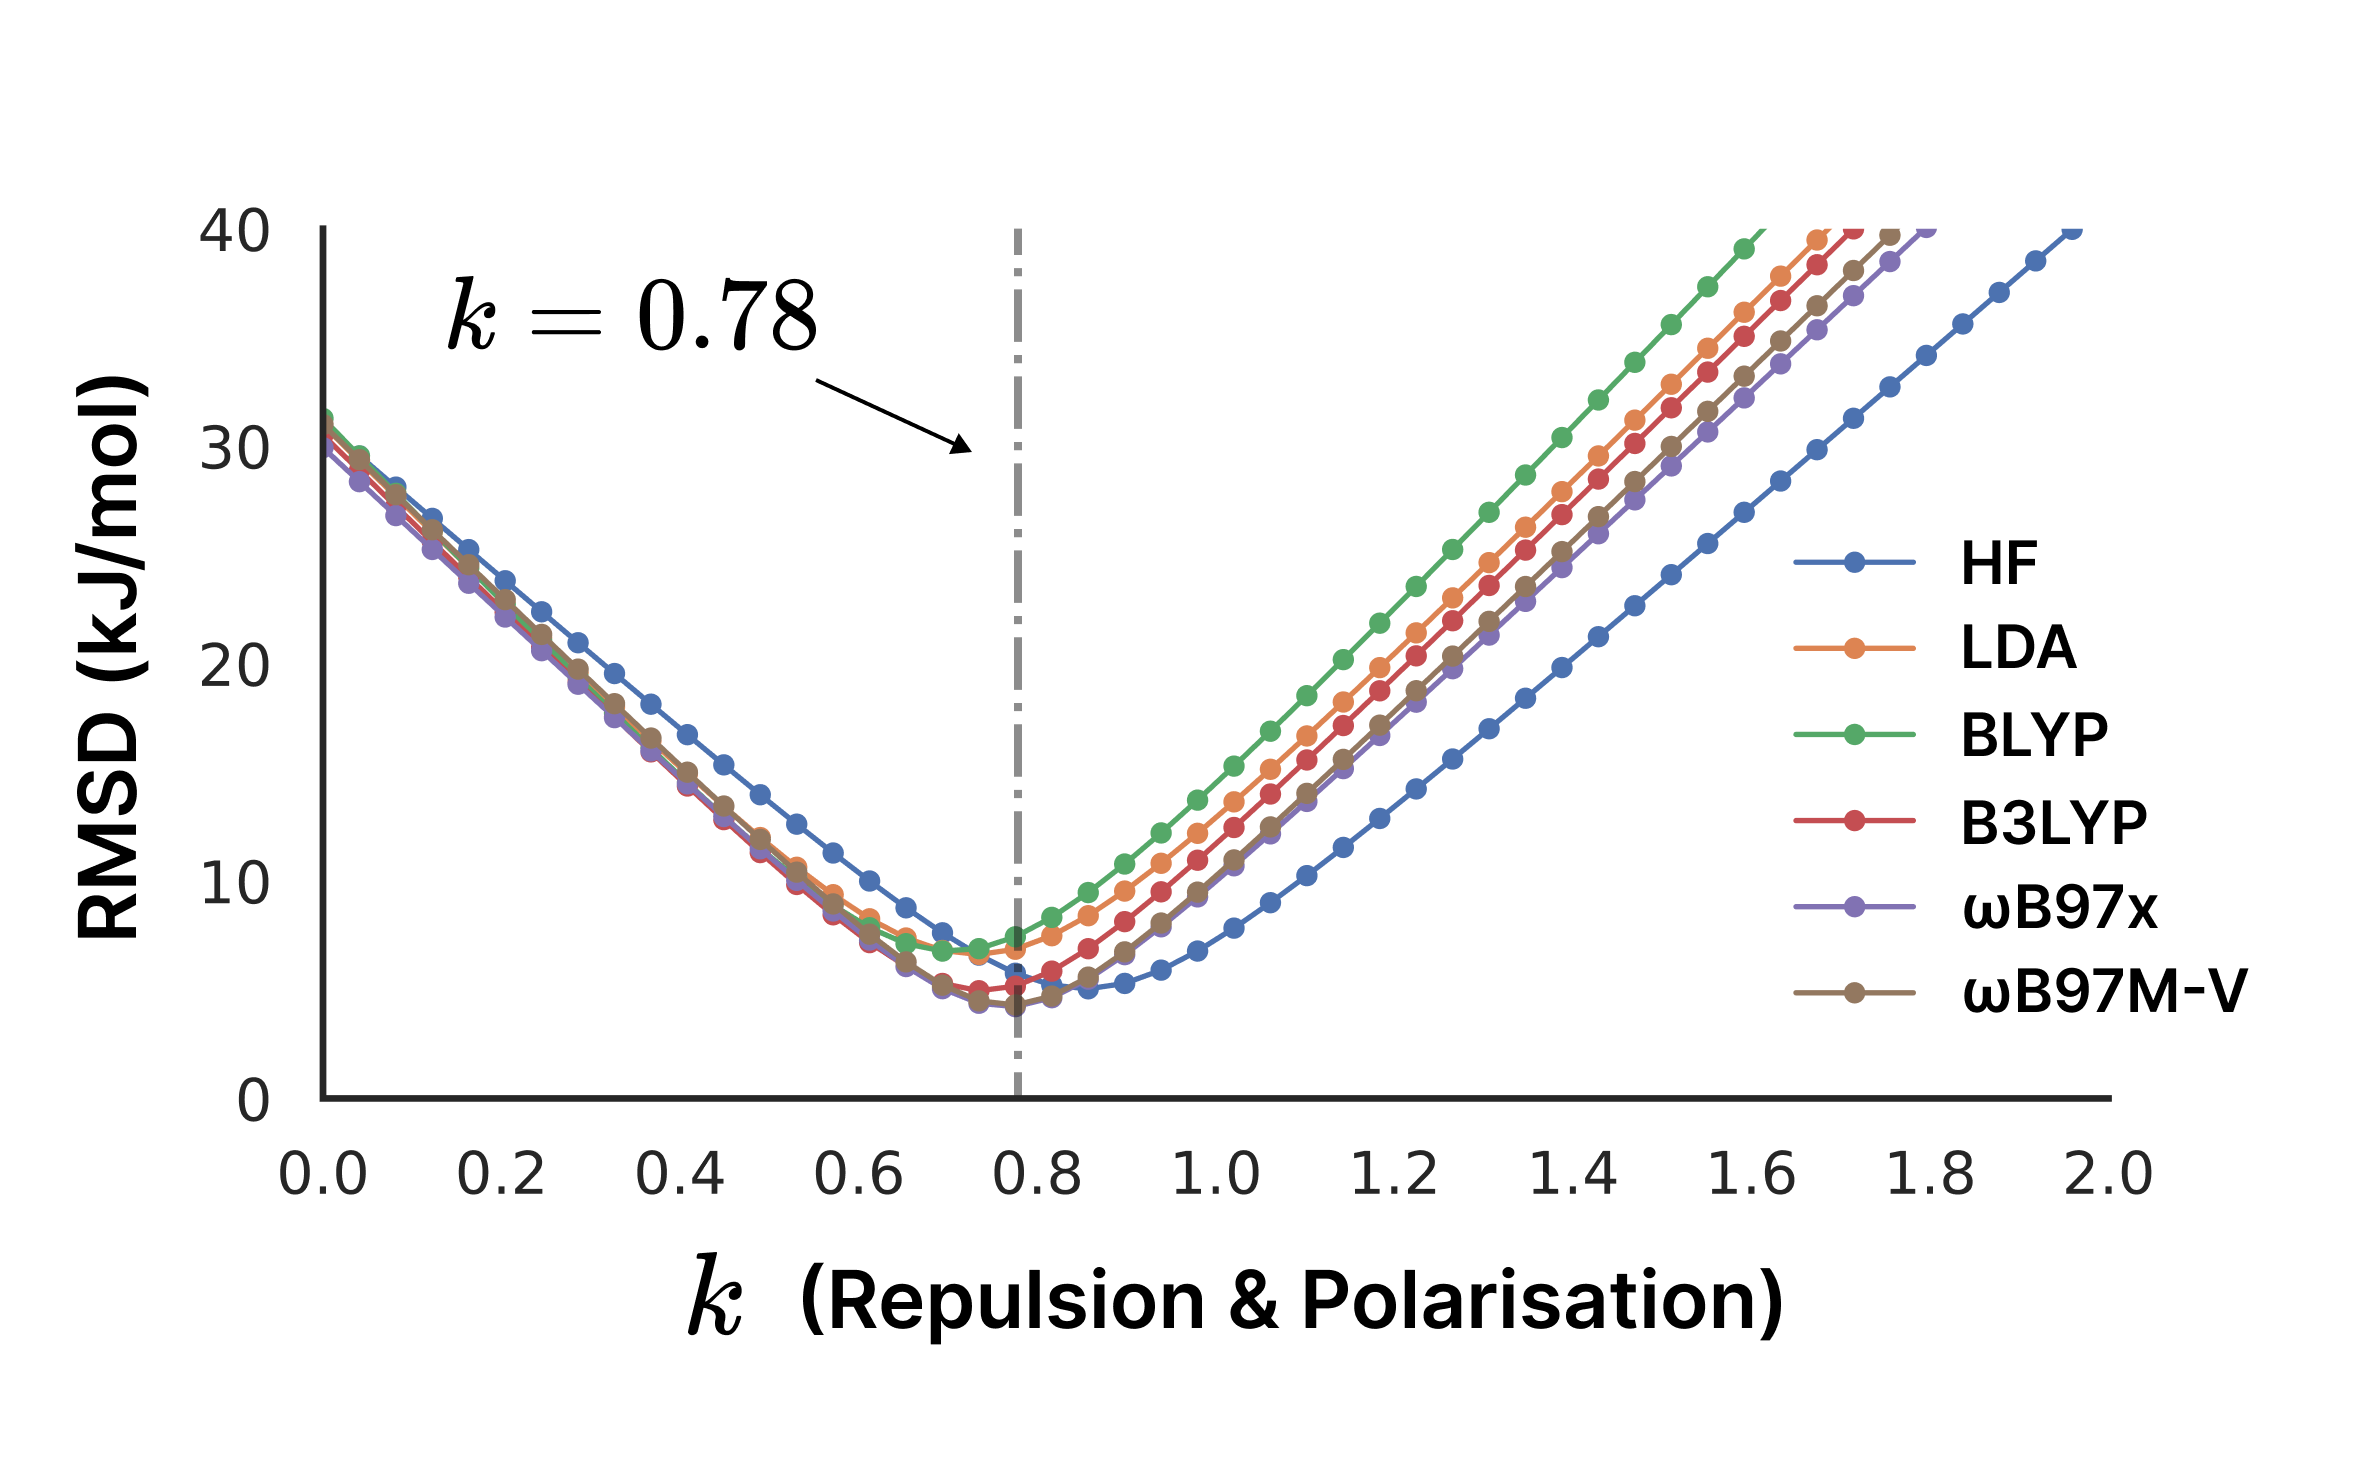
\includegraphics[width=0.9\textwidth]{figures/errors_ce1p.pdf}
    \label{fig:1_parameter_minima}
    \caption{Error distributions for HF, LDA, BLYP, B3LYP, $\omega$B97x and $\omega$B97M-V over a range of $k = k_\text{rep} = k_\text{pol}$ values.
    While there are clearly some differences between models, it should be seen that the minimum for $\omega$B97M-V at $k=0.78$ (highlighted by the
    grey dashed line) still produces good results for other models.}
\end{figure}

In the case of CE-1p, there is substantial agreement between different wavefunction sources for the optimal value of the fitted
$k$ parameter, with a minimum in the case of $\omega$B97M-V at $0.77850434\ldots$, i.e. $0.78$ (2 d.p.).
The only method with a significantly shifted minimum
value and is HF, but even there the difference between the RMSD of 5.0 kJ/mol for the optimal value ($k=0.86$) vs.
5.7 kJ/mol is less than 1 kJ/mol.

For the case of CE-2p all methods yield minima in a similar areas, and there is a region of the two-parameter space where the error is relatively flat
(plots are provided in the Supporting Information in Figure S2 % \ref{sifig:2_parameter_minima}
).
Given that, intuitively, $\omega$B97M-V should be the most accurate method against the reference (being the same method as used in the reference)
we elected to use two parameters from the minima of this approach, located at $k_\text{rep} = 0.485$ and $k_\text{pol} = 0.803$.
However, it must be pointed out that the agreement between the two-dimensional minima in CE-2p is much worse than in the one-dimensional case
of CE-1p which indicates its transferability to different molecular wavefunction sources is likely to be inferior.

The five-parameter model (CE-5p) was also examined, with scale factors fitted using least-squares,
and the resulting coefficients given in Table \ref{tab:5param}. For the five-parameter fit, values for all 
scale coefficients were fixed in the range $[0, 3]$, with the exception of $k_\text{rep}$, which was bounded from $[0.6,3]$.
These boundaries were introduced due to the potential for over-fitting - it was found that freely optimising the parameters
introduced negative scale factors or scale factors close to zero, with very small improvements to the errors for the model.
Based on the exploration of the parameter space for the CE-1p model, $k_\text{rep} \ge 0.6$ was chosen to allow enough
flexibility to alter the $k_\text{rep}$ parameter while constraining the fit to more (theoretically) reasonable parameters.
It can be seen here that the Coulomb scaling coefficient is very close to unity for all wavefunction sources, which is rationalised by 
the number of charged systems in the training set, where this will be the overwhelmingly dominant term for most of them.

\begin{table}
\caption{Fitted scaling coefficients for the different components in the CE-5p model
        when using the 6 different wavefunction sources explored in this work: HF, LDA, BLYP, B3LYP $\omega$B97X and $\omega$B97M-V.
        See equation \ref{eqn:ce_energy_model} for the relevant energy expression. Note that $k_\text{rep}$ values of 0.6
        correspond to the fixed lower bound in the least-squares fitting procedure.}
\label{tab:5param}
\centering
\begin{NiceTabular}{lrrrrrc}
\CodeBefore 
\Body
  \hline
Coefficient &    HF &   LDA &  BLYP &  B3LYP &  $\omega$B97X &  $\omega$B97M-V \\
\hline
$k_\text{coul}$ & 0.999 & 1.011 & 1.011 &  1.007 &  1.005 &  1.005 \\
$k_\text{exch}$ & 1.487 & 0.717 & 0.761 &  0.702 &  0.666 &  0.670 \\
$k_\text{rep}$  & 1.109 & 0.600 & 0.600 &  0.600 &  0.600 &  0.600 \\
$k_\text{pol}$  & 0.780 & 0.824 & 0.826 &  0.808 &  0.794 &  0.793 \\
$k_\text{disp}$ & 0.990 & 1.036 & 1.039 &  1.068 &  1.065 &  1.051 \\
\hline\\
\end{NiceTabular}
\end{table}

Error distributions for the training set are shown in Figure \ref{fig:kde_wavefunction_sources}, where it is notable that 
for all sources other than HF,  the five-parameter fit produces only negligible improvements
in overall energy errors relative to the transferable one and two-parameter fits, which coupled with the need to
introduce constraints is indicative that it's likely we are in the realm of overfitting. 
To further examine this, we must look outside the training set to evaluate the behaviour against external reference data.

\begin{figure}
    \centering
    \includegraphics[width=0.9\textwidth]{figures/merged_kde_training.pdf}
    \caption{Kernel density estimate plots showing the errors for the predicted energies vs.
    the reference ($\omega$B97M-V/def2-QZVP) dimer interaction energies in the training set when using the previous CE-B3LYP model, and GFN2-xTB, along with the 
    fitted CE-1p, CE-2p and CE-5p using the 6 wavefunction sources explored in this work
    (top to bottom): HF, LDA (SVWN5), BLYP, B3LYP, $\omega$B97X, $\omega$B97M with RMSD provided to the right of each plot.
    Each wavefunction source has been shifted in the y-axis to facilitate visual inspection of the distributions.}
    \label{fig:kde_wavefunction_sources}
\end{figure}

\subsection{S66$\times$8 set}

The primary use case for the proposed energy models, and indeed the major use case for the previous models, is for intermolecular interactions in organic molecular crystals \textit{i.e.}, intermolecular
interactions between neutral organic species. To this end, the S66x8 benchmark
set \cite{Rezac2011a,Rezac2011b,Brauer2016} constitutes an excellent test set to evaluate the performance of the fitted models over a range of intermolecular interaction distances, and understand its' behaviour for different interaction types. The overall results are shown in Table \ref{tab:S66x8_results}. Unsurprisingly, the previously fitted model (CE-B3LYP) performs very well for neutral systems, just as it did on the training set and in previous work. Likewise, across all fits, the B3LYP, $\omega$B97X and $\omega$B97M-V wavefunction sources are significantly better choices than HF, LDA and BLYP. This is not a surprising result, but it is consistent with intuition when it comes to the superior accuracy of (hybrid) DFT functionals.

Perhaps the most important conclusion from the results for this test set is that the five-parameter fits are only marginally better in performance (or sometimes worse) than the two-parameter fits.
The performance for $\omega$B97x and $\omega$B97M-V are almost identical - this is unsurprising when we consider how similar the models are in terms of their wavefunctions (the VV10 non-local correlation functional
has only been applied as a post-SCF correction).

\begin{table}
\caption{
Error Statistics for the S66x8 data set, showing Mean Absolute Deviation (MAD), Mean Signed Deviation (MSD) and Root-Mean-Square Deviation (RMSD) in kJ/mol, rounded to 1 decimal place.
}
\label{tab:S66x8_results}
\centering
\begin{NiceTabular}{lr|rrrrrr}
\CodeBefore 
\Body
\hline
{}  & {} & \Block{1-6}{CE-1p}\\
Statistic &  CE-B3LYP &  HF &  LDA &  BLYP &  B3LYP &  $\omega$B97X &  $\omega$B97M-V \\
\hline
MAD  &    2.4 &  3.3 &  2.6 & 2.6 &  2.1 &  2.0 &  2.0 \\
MSD  &   -0.8 & -3.1 & -0.4 & 1.2 &  0.2 & -0.5 & -0.5 \\
RMSD &    3.8 &  5.6 &  3.8 & 4.2 &  3.3 &  3.2 &  3.3 \\
\hline
{}  & {} & \Block{1-6}{CE-2p}\\
Statistic &  {} &  HF &  LDA &  BLYP &  B3LYP &  $\omega$B97X &  $\omega$B97M-V \\
\hline
MAD  &    {} &  3.7 &  2.2 & 2.3 &  2.1 &  2.1 &  2.1 \\
MSD  &    {} & -3.4 & -0.5 & 0.9 & -0.1 & -0.8 & -0.7 \\
RMSD &    {} &  6.9 &  3.7 & 3.7 &  3.3 &  3.6 &  3.5 \\
\hline
{}  & {} & \Block{1-6}{CE-5p}\\
Statistic & {} &  HF &  LDA &  BLYP &  B3LYP &  $\omega$B97X &  $\omega$B97M-V \\
\hline
MAD  &    {} &  1.7 &  2.6 &  2.8 &  2.0 &  1.7 &  1.8\\
MSD  &    {} & -0.1 & -1.7 & -1.5 & -0.8 & -0.5 & -0.4\\
RMSD &    {} &  2.7 &  4.6 &  5.0 &  3.5 &  2.9 &  2.9\\
\end{NiceTabular}
\end{table}


Similar to the results for the training set in the previous section, in Figure \ref{fig:kde_s66} it is apparent that more
parameters do not necessarily lead to wholesale improvement of the reliability of the models, and where they do, the improvement
is relatively minor when considering potential applications to non-covalent interactions. The best result for CE-5p, for
example, was actually HF with an RMSD of 2.5 kJ/mol vs. the best result for CE-1p being $\omega$B97X with
an RMSD of 3.2 kJ/mol. This is not totally insignificant, but when put in the context of the training data and the 
kinds of interactions that are present in the S66x8 dataset, and the difference between 5 parameters (that may be
less transferable) and only a single parameter we believe the trade-off of around 0.5 kJ/mol (which largely corresponds to a shift
in mean error) is worthwhile.

With few exceptions (BLYP \& HF in some cases), the error distributions are largely symmetric about zero, though there are 
longer and denser tails in the over-binding direction, which may be explained through the trends at different intermolecular
separations in the S66x8 set. Once again, in this context the B3LYP, $\omega$B97M-V and $\omega$B97x methods are clearly superior 
in their reliability, particularly for the more transferable CE-1p model.

It is worth comparing our results with the recently published $\omega$B97X-3c composite method \cite{Muller2023}, which has
also been evaluated against the S66 set (i.e. the subset of the S66x8 set with separation scale factor $r = 1.0$) 
In \cite{Muller2023}, $\omega$B97X-3c had a MAD of roughly 1.2 kJ/mol over these interactions, compared to say the corresponding
$\omega$B97X variant of the CE-1p model at roughly 1.8 kJ/mol (the corresponding value for CE-B3LYP is 2.5 kJ/mol). Likewise, a natural comparison method for the approach are the SAPT(DFT) and SAPT0 methods, for which the corresponding MAD values, taken from \cite{Xie2022}, are 1.4 kJ/mol for SAPT(DFT) and 4.1 kJ/mol for SAPT0. 
A full list of the MAD values for the S66 set is provided in the Supporting Information in Table S4 %\ref{sitab:s66_mean_deviations}
.
We believe this represents excellent agreement considering the relative cost of the methods, with our model not requiring an SCF
for the combined dimer wavefunction.

\begin{figure}
    \centering
    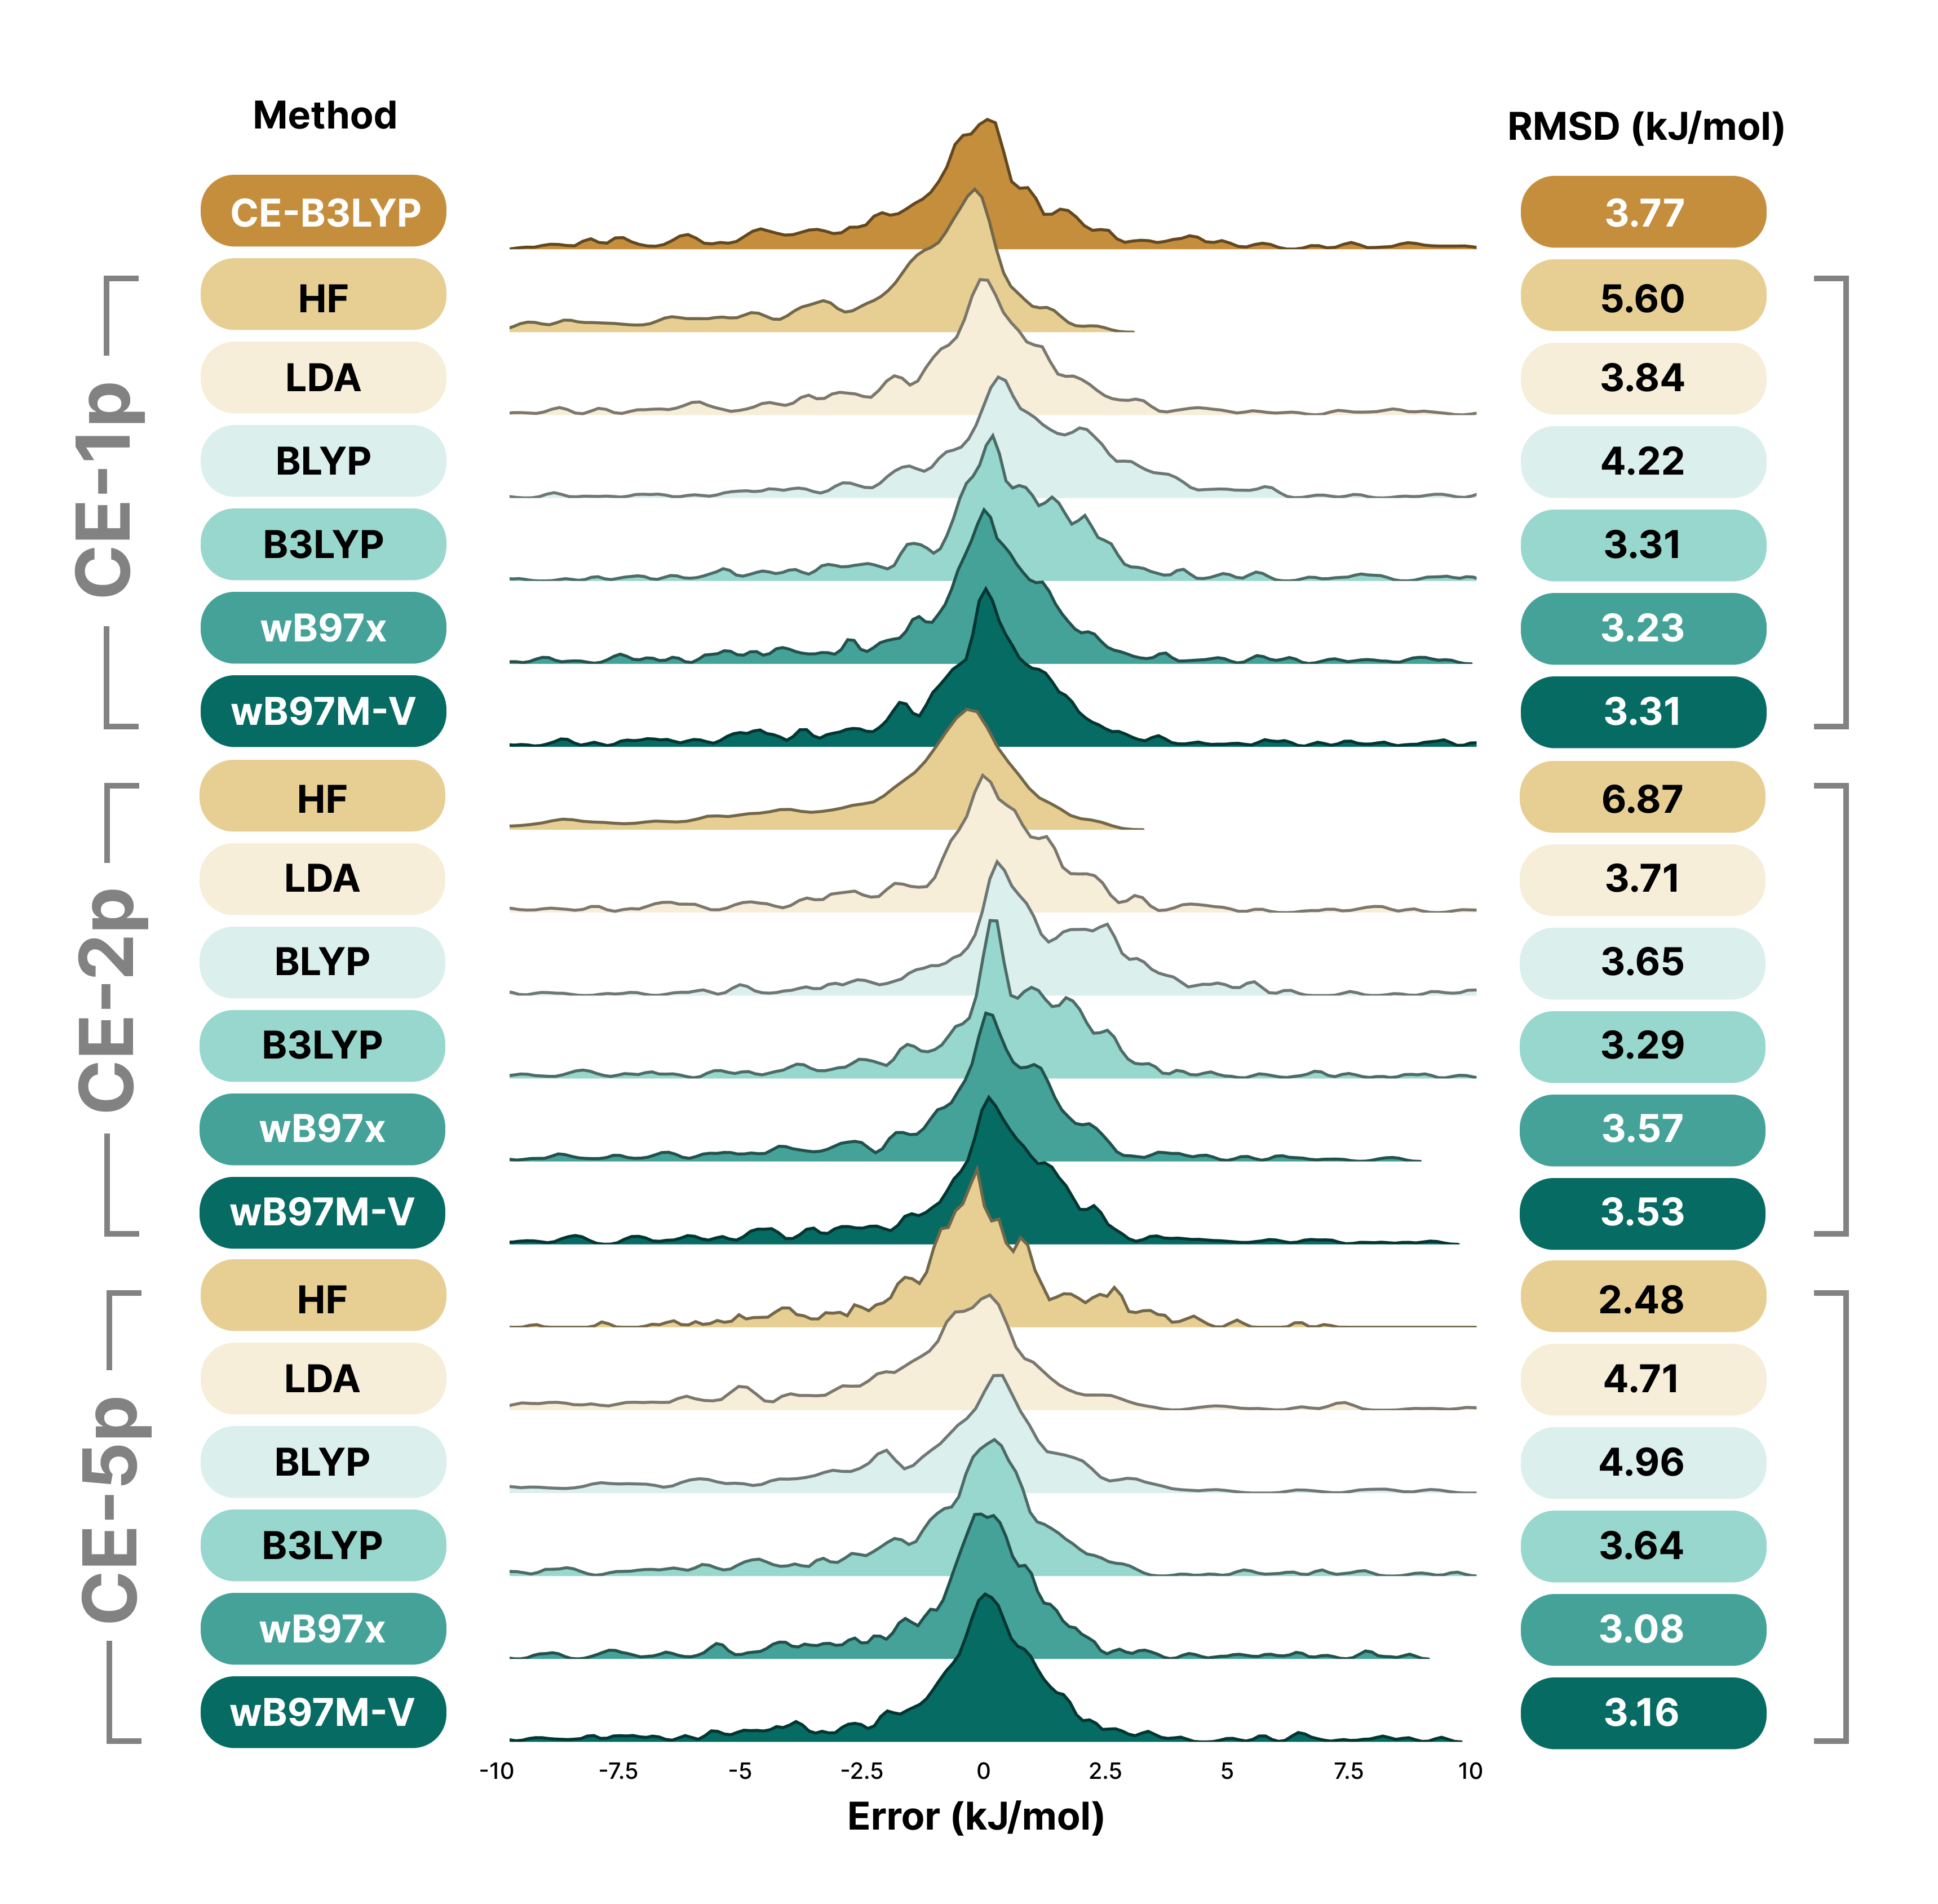
\includegraphics[width=0.9\textwidth]{figures/merged_kde_s66.pdf}
    \caption{Kernel density estimate plots for the S66x8 set using the CE-1p, CE-2p and CE-5p fits,
    the previous CE-B3LYP model, and the 6 wavefunction sources used in this work (top to bottom): 
    HF, LDA (SVWN5), BLYP, B3LYP, $\omega$B97X, $\omega$B97M-V with RMSD provided on the right-hand side of each plot. Each 
    wavefunction source has been shifted in the y-axis to facilitate visual inspection of the distributions. }
    \label{fig:kde_s66}
\end{figure}

\subsection{Trends in error vs. separation distance}

In the context of molecular crystals, it is of course important for dimer interaction energies to be accurate over a range 
of intermolecular separations. Furthermore, characterisation of the kinds of errors and trends with distance and interaction 
type give insight into where models are accurate
and where their accuracy may be limited - be it systematic or otherwise.

Careful examination of Figure \ref{fig:s66_error_vs_sep} shows the distribution of errors surrounding the mean error when using 
the CE-5p fit is marginally narrower, but it appears the CE-5p fit is indeed over-fitted, as its systematic 
over-binding at closer than equilibrium intermolecular separations (0.9, 0.95 in the separation scale) is more extreme than for
both the previous CE-B3LYP model and the CE-1p model. 
This trend, coupled with the marginal difference in overall performance for the CE-1p fit \textit{vs.} the CE-5p fit 
(3.3 kJ/mol for CE-1p using B3LYP \textit{vs.} 2.5 kJ/mol RMSD for the best CE-5p model, which was using HF) is,
in our judgement, enough to recommend usage of the CE-1p model, with only a single free parameter that is clearly 
transferable across wavefunction sources.


\begin{figure}
    \centering
    \includegraphics[width=0.9\textwidth]{figures/s66_trends_b3lyp.pdf}
    \caption{Trends in errors across different scaled separations for the S66x8 benchmark set when 
    using different models in this work: CE-B3LYP (top),  and the CE-1p (upper middle), 
    CE-2p (lower middle) and CE-5p (bottom) for the B3LYP wavefunction source. 
    The solid lines indicate the mean error value, while the shaded region represents the 95\% confidence interval.
    The separation scale is relative to the equilibrium separation i.e. a value of 1.0 is at equilibrium, while a
    value of 0.9 is 90\% of the equlibrium separation. Values between explicitly
    calculated separations (0.9, 0.95, 1.0, 1.05, 1.1, 1.25, 1.5, 2.0) have been linearly interpolated in order
    to show the behavioural trends.}
    \label{fig:s66_error_vs_sep}
\end{figure}

Errors at closer-than-equilibrium separations are of particular relevance to high-pressure studies of molecular crystals, and
previous work \cite{Eikeland2017} has shown that the CE-B3LYP model demonstrated significant errors compared to counterpoise-corrected B3LYP 
calculations on dimers in hydroquinone clathrates of methanol and acetonitrile. This was at least partly attributed to 
the $k_\text{exch-rep}$ scaling coefficient affecting repulsion at close separations. To examine this behaviour with the now larger repulsion scaling parameter for the CE-1p model relative to the previous CE-B3LYP model
($k=0.78$ vs. $k_\text{exch-rep}=0.6177$), we evaluated dimer interaction energies for the same
systems as in \cite{Eikeland2017} when using $\omega$B97M-V/def2-svp as the wavefunction source.
The results of these calculations, comparing CE-B3LYP, CE-1p and GFN2-xTB are summarised in the Supporting Information in Figures S3 %\ref{sifig:hq_pressure} 
and S4 %\ref{sifig:hq_pressure_correlations}
. 
The results were mixed; some systems showed improvements over the previous CE-B3LYP model, others did not. The CE-1p
model cannot be said to be an improvement in this regard over the old model, but neither can it be said to be worse. 
This is indicative that, despite previous discussion in \cite{Eikeland2017} the errors are not solely associated with the repulsion 
scale factor, as there is a significant interplay between the dispersion damping
coefficients as well. Ultimately, if we wish to have an improved model at closer intermolecular separations then, at a minimum, 
the training data set would need to be re-examined - along with changes likely being required in the assumptions of the model
(e.g. a departure from global scaling parameters) which is outside the scope of this work.
However, it is worth emphasising that as interactions get stronger at closer separations we should expect that errors get larger
for almost any method - and that the present model, where we are assuming relatively little deformation in
the molecular electron density, will eventually break down at close enough separations where significant overlap between 
monomer wavefunctions becomes a reality.

\section{Lattice energies for molecular crystals}

The previous CE models, particularly CE-B3LYP, have already been successfully applied to the prediction of lattice energies for
neutral molecular crystals via the direct summation technique. Prediction of such lattice energies is particularly challenging, 
due to the interplay of intermolecular interactions over a 
variety of distances where systematic errors will tend to manifest themselves largely as wrong absolute values for the lattice energies.
At present, the X23 benchmark set \cite{Reilly2013, Dolgonos2019}
(itself an extension of the C21 set \cite{Otero-de-la-Roza2012b}) constitutes the most reliable and robust set of reference values
for molecular crystal lattice energies. 

Table \ref{tab:x23_results} shows the resulting error statistics in lattice energies for the models explored in this work,
compared with those for the CE-B3LYP model. Optimised geometries that were previously used in the X23 revised
benchmark \cite{Dolgonos2019} were used, as well as experimental geometries with normalised hydrogen bond lengths;
the results for the experimental geometries are available in the Supporting Information in Table S7 %\ref{sitab:x23_results_exp_norm}
.
It is worth noting when interpreting these data, that the standard error ($\sigma$) for sublimation enthalpies is typically in the range of
4 kJ/mol \cite{Chickos2003}, and the correction procedure involving vibrational contributations to the sublimation enthalpy will further introduce
its own errors.
It is also worth highlighting that 6 of the molecules in the X23 set are present in the training set,
namely urea (UREAXX), benzene (BENZEN01), imidazole (IMAZOL13), formamide (FORMAM02), succinic acid (SUCACB09) and uracil (URACIL). However,
the training set is based on only the nearest dimers (rather than the dozens or hundreds of contributing energies to the lattice energy) 
and using a different reference method than in the reference X23 data. 

It can be seen in Table \ref{tab:x23_results} that the errors for different models are nowhere near as uniform as they were for the S66x8 benchmark set.
This should not be surprising - any systematic over- or under-estimation for interactions will be amplified when summing across many interactions/dimer pairs. The transferable, single parameter model demonstrates excellent performance and transferability across different wavefunction methods, though the success is
significantly diminished when examining the HF results.


\begin{table}
\centering
\caption{
Error Statistics for the X23 data set, showing Mean Absolute Deviation (MAD), Mean Signed Deviation (MSD) and
Root-Mean-Square Deviation (RMSD) in kJ/mol for the CE-1p, CE-2p and
CE-5p models investigated in this work, along with the GFN2-xTB method 
(calculated using the same direct summation of dimer energies method). 
All values here are calculated using the PBE0+MBD/light optimised geometries used in \cite{Dolgonos2019}, for
corresponding values on the experimental geometries see the Supporting Information Table S7 %\ref{sitab:x23_results_exp_norm}
}
\label{tab:x23_results}
\begin{NiceTabular}{lr|rrrrrr}
\CodeBefore
\Body
\hline
{}  & {} & \Block{1-6}{CE-1p}\\
Statistic &  CE-B3LYP &  HF &  LDA &  BLYP &  B3LYP &  $\omega$B97X &  $\omega$B97M-V \\
\hline
MAD  &     7.3 &  18.4 &   4.3 &    4.7 &     3.6 &     5.2 &     5.9 \\
MSD  &    -6.3 & -18.4 &  -2.8 &    3.0 &    -1.0 &    -4.1 &    -4.9 \\
RMSD &     9.7 &  23.2 &   5.8 &    5.6 &     4.8 &     7.1 &     7.6 \\
\hline
{}  & {} & \Block{1-6}{CE-2p}\\
Statistic &  GFN2-xTB &  HF &  LDA &  BLYP &  B3LYP &  $\omega$B97X &  $\omega$B97M-V \\
\hline
MAD  &     11.2 &  21.0 &   6.0 &    4.7 &     6.3 &     8.2 &     7.9 \\
MSD  &     -7.6 & -20.9 &  -4.2 &    1.3 &    -3.4 &    -6.7 &    -6.7 \\
RMSD &     15.2 &  27.6 &   7.7 &    5.6 &     8.4 &    11.2 &    10.9 \\
\hline
{}  & {} & \Block{1-6}{CE-5p}\\
Statistic & {} &  HF &  LDA &  BLYP &  B3LYP &  $\omega$B97X &  $\omega$B97M-V \\
\hline
MAD  &     {} &  5.4 &  12.0 &   13.2 &     9.5 &     7.3 &     7.4 \\
MSD  &     {} & -3.6 & -11.5 &  -12.7 &    -9.1 &    -6.7 &    -6.8 \\
RMSD &     {} &  8.1 &  14.0 &   15.6 &    11.8 &     9.6 &     9.7 \\
\end{NiceTabular}
\end{table}

There is little doubt that the accuracy of the models presented here, when using direct summation for the lattice energies is 
reliant on cancellation of errors (though the same may be said for all other methods). Nevertheless, the results for
the CE-1p model using B3LYP, with a MAD of only 3.6 kJ/mol compares very favourably with the current 
state-of-the-art \cite{Price2023}, where the \emph{best} method 
(a composite of B86bPBE-25-XDM//B86bPBE-XDM approach including a basis set correction) reported had a MAD of 2 kJ/mol. 
For comparison, the same work reported PBE0-MBD giving a MAD of 3.5 kJ/mol when using the `Tight' basis set.

Relative behaviour of the CE-1p, CE-2p and CE-5p models when using the B3LYP
functional against CE-B3LYP may be seen in Figure \ref{fig:x23_errors}, which indicates that the
single-parameter model is an improvement over the alternatives across almost every system. The results for cytosine indicated that there
may be some systematic error in the models, which merited further investigation into polarisation, as discussed in the next sub-section. 

\begin{figure}
    \centering
    \includegraphics[width=0.95\textwidth]{figures/X23_line_plot.pdf}
    \caption{Errors in predicted X23 energies (difference from reference values) for the CE-B3LYP (grey, dotted line) and the 
    CE-1p (blue), CE-2p (orange) and CE-5p (black) models using B3LYP/def2-SVP as the wavefunction
    source. The overall error statistics for all models are given in Table \ref{tab:x23_results}. All
    values here are calculated using the PBE0+MBD/light optimised geometries used in \cite{Dolgonos2019}, for
    corresponding values on the experimental geometries see the Supporting Information Table S7 %\ref{sitab:x23_results_exp_norm}
    }
    \label{fig:x23_errors}
\end{figure}

\subsection{Crystal polarisation effects}

There are several sources of possible error in the direct summation method used here for lattice energies, 
with one of the more significant sources of error being the treatment of polarisation. In a crystalline environment, 
the framework utilised in the CE energy models assumes that the polarisation contributions are pairwise additive. 
However, the true polarisation energy is fundamentally many-body in nature, due to the quadratic dependence on magnitude
of the electric field:

\begin{equation}
    \label{eqn:crystal_polarisation}
    E_\text{pol}^i = -\frac{1}{2} \alpha_i | \overrightarrow{F}_i |^2  
\end{equation}

Here $i$ is the $i$-th atom, $\alpha_i$ is its' polarisability, $E_\text{pol}^i$  is the polarisation energy for this atom,
and $\overrightarrow{F}_i$ is the electric field at atom $i$ from its' environment, either from the neighbouring monomer
(in the case of a pair) or from the crystal environment. While the field is just the pairwise sum over neighbours, the 
square of this quantity is no longer separable. 

\begin{figure}
    \centering
    \includegraphics[width=0.95\textwidth]{figures/X23_line_plot_cpol.pdf}
    \caption{Errors in predicted X23 energies (difference from reference values) for the CE-1p method using B3LYP/def2-SVP
    as the wavefunction source when using two different polarisation models. 
    Here `Pairwise field' corresponds to the usual method of calculating the polarisation
    term for the lattice energy, i.e. each pair is calculated individually, whereas `Crystal field' evaluates the electric
    field from all neighbours at the atomic positions of the symmetry-unique molecule(s) in the crystal. See equation \ref{eqn:crystal_polarisation}.}
    \label{fig:x23_cpol}
\end{figure}

The practical difference in the case of crystals may be seen in Figure \ref{fig:x23_cpol}, where the sum of pairwise polarisation terms
overestimates the polarisation energy of the crystal, especially for cytosine. In contrast, summing the field experienced by a monomer
over all interactions in the crystal before computing the polarisation energy significantly improves most energies for the X23 data set.
It should be noted that there is a further effect from using gas phase wavefunctions, that may lead to underestimation of the polarisation
in comparison to corresponding wavefunction in the solid-state.
Since gas-phase wavefunctions are used throughout the current procedure, 
we are likewise underestimating the polarisation of the initial molecular wavefunction. These two factors will compete and we may (or may not)
experience cancellation of errors, but this is an aspect that must be understood if, moving forward, molecule-in-crystal wavefunctions, for
example, were to be used with this energy model to estimate lattice energies. 

For now, we can examine the influence of evaluating the polarisation energy using the theoretically more correct approach of summing
over contributions to the field before computing the energy. This manifests in changes in the error statistics:
the MAD value shifts to 4.4 kJ/mol (vs. 3.6 kJ/mol), largely due to the systematic shift in MSD to 2.2 kJ/mol (vs. -1.0 kJ/mol) 
while the RMSD only shifts to 5.3 kJ/mol (vs. 4.8 kJ/mol). 


This suggests that if the goal is to predict relative lattice energies, as it so often is in the context of molecular crystals, then using a polarisation term based on the electric field of the crystal should be considered. 
Indeed, there is a minor increase in error (less than 1 kJ/mol) for the
absolute values of the lattice energies when compared to reference values, but the errors are 
likewise more systematic which tends to improve relative energies.
Furthermore, in ionic systems, the effects of the pairwise approximation for polarisation are even greater. An illustrative example is cubic \ce{NaCl}, which has has zero net electric field at the ion positions, but when calculated pairwise there is an erroneous net polarisation energy of around 400 kJ/mol.  

\section{Conclusions}

We have implemented, fitted and demonstrated the accuracy of a new single parameter 
intermolecular interaction energy model, CE-1p, which
is transferable across different wavefunction sources. The model constitutes an
excellent accuracy/computational cost trade-off, with a MAD of 2.0 kJ/mol across the S66x8
benchmark set, and near state-of-the-art performance when predicting lattice energies for the X23
benchmark set, with a MAD of 3.6 kJ/mol, while using the simplest pairwise sum in real space.
While there is little
doubt that this model (and others) exhibit error cancellation, we believe it constitutes an 
efficient and accurate method for quantitative predictions of intermolecular interactions which 
may \emph{also} be rationalised and understood through sensible separation of the energy into
distinct contributions.

We have also examined the performance of the GFN2-xTB tight binding model as a rapid method for 
similar purposes, with only relatively minor loss in accuracy for dimer energies in organic
neutral systems. In particular, for neutral organic molecules (which constitute a large part of
the chemical systems of interest in molecular crystals) using GFN2-xTB through visualisation 
software such as CrystalExplorer provides near instant feedback and allows for real-time 
exploratory evaluations, as in most cases it is 1-2 orders of magnitude faster than our energy
model.


Our recommendation for the end-user of these methods, who wishes to rationalise the
intermolecular interactions in a molecular crystal is as follows:
\begin{itemize}
    \item First, calculate the interaction energies using GFN2-xTB, which is extremely low cost for pairwise interactions. Particularly, it is worth examining interactions beyond nearest-neighbours using such methods, as their long-range behaviour should be reliable. These can be visualized using energy frameworks \cite{Turner2014}. 
    \item Calculate the same energies using the CE-1p model, using B3LYP, $\omega$B97x or $\omega$B97M-V functionals, depending on which is available in your QM software of choice.
    \item If these models are not in agreement with respect to the relative strength of interactions, it warrants further detailed investigation with higher-level methods.
    \item If lattice energies are of interest, strongly consider the polarity of the molecule(s) in your system, and whether or not the pairwise approximation for polarisation is appropriate.
\end{itemize}

There are several avenues for further improvements and developments, including: 
\begin{itemize}
    \item The possibility of fitting a model using DFT exchange-correlation rather than HF exchange due to the reduction in computational cost over evaluating the exact exchange matrices for the two monomers ($A$ and $B$) and the better scaling speed-ups available for the Coulomb term, particularly if overall accuracy of the model is not sacrificed.
    \item Departing from global scaling parameters - particularly at close intermolecular separations, though this would be a significant change in the model.
    \item Examination of the connection between the orthogonalised electron population (see Supporting Information Section S9 %\ref{sisec:overlap_repulsion}
    ) and the repulsion and exchange terms for development of low-cost approximations.
\end{itemize}

In summary, the new single-parameter CE-1p model is generally more accurate, significantly more transferable (not only to other wavefunction methods but in its coverage of more of the periodic table, which enables application to more chemical problems), and has (qualitatively) a more sound theoretical basis than the existing CE-B3LYP model. Hence, we view it as an excellent replacement for the previous method, which will no doubt find broad application across a variety of chemical problems, particularly in the domain of molecular crystals. This work has been implemented and is already available in the open source software `occ' made available on GitHub 
(\url{https://github.com/peterspackman/occ})
The incorporation of the newly proposed CE-1p model, along with access to GFN2-xTB will be available in a forthcoming release of CrystalExplorer where we are optimistic both will be valuable additions for the community. 


     %-------------------------------------------------------------------------
     % The back matter of the paper - acknowledgements and references
     %-------------------------------------------------------------------------

     % Acknowledgements come after the appendices

\ack{Acknowledgements}

JDG thanks the Australian Research Council for funding under grant FL180100087. PRS and JDG thank the Pawsey Supercomputing Centre and National Computational Infrastructure for provision of computing resources. 

     % References are at the end of the document, between \begin{references}
     % and \end{references} tags. Each reference is in a \reference entry.

%% Note added by Overleaf: If using bibtex, remove the "references" environment above, and uncomment the following line.
\referencelist{iucr}



\end{document}                    % DO NOT DELETE THIS LINE
%%%%%%%%%%%%%%%%%%%%%%%%%%%%%%%%%%%%%%%%%%%%%%%%%%%%%%%%%%%%%%%%%%%%%%%%%%%%%%
